\documentclass[12pt,a4paper,oneside]{article}

\usepackage[czech]{babel}
\usepackage[utf8]{inputenc}
\usepackage[T1]{fontenc}
\usepackage{lmodern}
\usepackage{graphicx}
\usepackage{wrapfig}
\usepackage{hyperref}
\usepackage{listings}

\bibliographystyle{ieeetr}  

\begin{document}
\def\refname{Literatura}
\lstset{language=Ruby}

\title{Ruby}
\author{Pavel Pokorný}
\date{\today}
\maketitle

%%%%%%%%%%%%%%%%%%%%%%%%%%%%%%%%%%%%%%%%%%%%%

Ruby je dynamický jazyk se zaměřením na jednoduchost a produktivitu. Elegantní syntaxe se přirozeně čte a jednoduše píše. Toto tvrzení jsem převzal z oficíální webové stránky jazyka Ruby a mohu jen souhlasit. I velice složité věci je možné v napsat v tomto jazyce s nebývalou elegancí. Co se zdá na první pohled jednoduché, nemusí být ale jednoduché pod povrchem, což dokazují i slova tvůrce tohoto jazyka. Pro vytvoření tak použitelného a přístupného jazyka jako je Ruby musel Yukihiro Matsumoto vynaložit obrovské úsilí.

\begin{quotation}
,,Ruby je jazyk jednoduchý navenek, ale uvnitř je velice komplexní, stejně jako lidské tělo.'' 

\em{Yukihiro 'Matz' Matsumoto, tvůrce Ruby}
\end{quotation}

V tomto článku jsou popsány základy objektového modelu, spustitelných objektů a možnosti metaprogramování v jazyce Ruby.

Metaprogramování je psaní kódu, který nějakým způsobem za běhu programu manipuluje s konstrukcemi jazyka. Ruby přímo vyzývá svými vlastnostmi k metaprogramování, vše může být vytvořeno nebo změněno za běhu programu. Programátor má tedy velikou volnost a takřka neomezené možnosti, ale s tím přichází i větší zodpovědnost. Není těžké 'rozbít' základní funkčnost vestavěných tříd a objektů a taktéž při použití jakékoliv knihovny je možné redefinovat kteroukoliv z poskytovaných funkčností. Od programátora se tedy předpokládá jakási ukázněnost a je na něj převedena veškerá zodpovědnost. Na oplátku získává volnost a možnost si vše přizpůsobit či rozšířit.

Nejspíše i kvůli těmto vlastnostem jazyka lpí komunita Ruby vývojářů tak moc na otestovaném kódu. Mnohdy kód bez testů jako by ani nebyl. Když už jsem se zmínil o komunitě, je tu ještě jedna věc - a sice podpora open source software. Sdílet zdrojový kód a nechat kohokoliv na světě ho volně užívat a popřípadě vylepšovat je zkrátka trend a Ruby vývojáři můžou jít ostatním jen příkladem. Většina projektů využívá server GitHub, který nabízí pro open source projekty zdarma hosting verzovacího systému Git, správu issues, wiki a vestavěné sociální prvky, což vystihuje podtitul '\emph{social coding}'. GitHub se zkrátka stává Facebookem pro programátory.

V článku předpokládám, že má čtenář základní znalosti jazyka Ruby, pokud tomu tak není, doporučuju si projít nespočet online tutoriálů nebo skvělou knihu {\it Eloquent Ruby} \cite{olsen2011eloquent}, která obsahuje také velkou sekci o metaprogramování. Mnoho užitečných informací jsem se dozvěděl také v knize {\it Metaprogramming Ruby} \cite{metaRuby}, která pokrývá pokročilejší vlastnosti tohoto jazyka a obsahuje mimo jiné spoustu zažitých vzorů řešení různých problémů (v knize jsou nazývány tyto vzory jako kouzla - \emph{spells}).

%%%%%%%%%%%%%%%%%%%%%%%%%%%%%%%%%%%%%%%%%%%%%

\section{Základní struktury jazyka}

Vše je objekt, je tedy rozumné začít u něj. Objekt v Ruby je na první pohled jednoduchá struktura, obsahuje své metody, proměnné, referenci na svou třídu a unikátní identifikátor (\emph{object\_id}).

Podobně jako v jiných objektově orientovaných jazycích obsahuje \textbf{instanční proměnné} a narozdíl od statických proměnných nejsou instační proměnné závislé na třídě objektu. Proměnná objektu je vytvořena, když je jí přiřazena hodnota. Můžou tedy existovat objekty stejné třídy obsahující úplně jiné instační proměnné. Seznam instančních proměnných objektu je možné získat od každého objektu zavoláním metody \emph{instance\_variables}, jednotlivé proměnné pak pomocí \emph{instance\_variable\_get} a \emph{instance\_variable\_set}.

Jak se dá předpokládat, objekty mají \textbf{metody}, které je možné zavolat na daném objektu. Objekty dědí metody ze svého tzv. \emph{ancestors chain}. Metody však nejsou uloženy přímo v objektu samém, ale v třídě daného objektu (což je objekt třídy \emph{Class}). Seznam metod, které má objekt k dispozici, je možné získat metodou \emph{methods} nebo variantami \emph{instance\_methods}, \emph{singleton\_methods}.

\textbf{Třídy} jsou také objekty a vztahují se k ním stejná pravidla jako k objektům. Třídy mají také svou třídu, která se nazývá \emph{Class}, a mají také metody, které budu dále označovat jako třídní metody. Třída \emph{Class} není v hierarchii na vrcholu, dědí od třídy \emph{Module}. Třída je tedy modul, který obsahuje některé důležité metody navíc (\emph{new}, \emph{allocate}, \emph{superclass}), díky kterým lze vytvořit její instanci. Každá instance třídy \emph{Class} (tedy každá třída) je potomkem třídy \emph{Object}, která je potomkem třídy \emph{BasicObject}. \emph{BasicObject} je opravdovým vrcholem v objektovém modelu jazyka Ruby. Není těžké se v tomto světě propletených tříd a objektů ztratit, k pochopení snad přispěje ilustrace \ref{fig:object_model}, ke které se dostaneme ke konci článku.

\textbf{Moduly} a třídy jsou úzce spjaty a v mnoha případech jsou zaměnitelné. Moduly jsou používány, když je kód určen k vložení do jiných metod a mluvíme pak o tzv. \emph{code mixins}. To zvyšuje znovupoužitelnost takového kódu. Druhou funkcí modulů je organizace kódu do tzv. \emph{namespaces}, což jednak brání kolizím v názvech tříd a dovoluje seskupovat logicky související metody, třídy a konstanty. Třídy jsou používány, pokud je třeba vytvářet instance nebo využívat dědičnost.

Reference na objekty jsou udržovány v proměnných a protože třídy a moduly jsou také objekty, je nutné reference na ně také někde udržovat. Reference na třídy a moduly jsou \textbf{konstanty}, což jsou v Ruby všechny názvy začínající velkým písmenem. Všechny konstanty jsou uspořádány do stromu, kde uzly jsou konstanty ukazující na třídy a moduly a listy ukazují na ostatní konstanty.

Když je zavolána \textbf{metoda}, vyhledá ji Ruby interpret v \emph{ancestors chain}, tedy ,,šňůře'' tříd začínající třídou objektu a končící třídou \emph{BasicObject}. O volání metod se můžeme vyjadřovat jako o zasílání zpráv, příjemce budiž tedy objekt, jehož metoda byla zavolána. Tento přístup je v ruby přirozený, každý objekt má metodu \emph{send}, kterou je možné mu zaslat zprávu i s případnými parametry. Když interpret nalezne metodu, nastaví příjemce jako aktuální objekt (který je vždy možné získat klíčovým slovem \emph{self}) a spustí kód metody. Pokud není explicitně uveden příjemce, interpret předpokládá, že se jedná o metodu objektu \emph{self} a taktéž instanční proměnné hledá u tohoto objektu. Každý kousek Ruby kódu je vykonáván v prostředí nějakého
\begin{wrapfigure}{r}{6cm}
\centering
\setlength\fboxsep{0.5pt}
\setlength\fboxrule{0.5pt}
\fbox{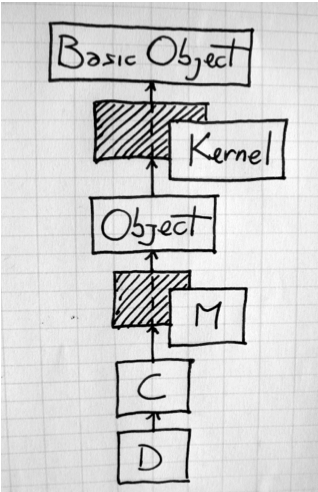
\includegraphics[width=0.3\textwidth]{figures/included_modules.png}}
\caption{Moduly \emph{Kernel} a \emph{M} vložené do \emph{ancestors chain} objektů třídy D \cite{metaRuby}}
\label{fig:included_modules}
\end{wrapfigure}
objektu a tento aktuální objekt lze získat klíčovým slovem \emph{self}. Při definici nové třídy zastává roli \emph{self} právě definovaná třída. V tělech metod je \emph{self} objektem, na kterém byla metoda volaná. V kontextu nejvyšší úrovně zastává roli \emph{self} objekt nazvaný \emph{main}, který je automaticky vytvořen Ruby interpretem. Object \emph{main} je speciální také tím, že metody vytvořené v jeho kontextu jsou uloženy jako privátní metody třídy \emph{Object} a jsou tak jednoduše přístupné všem objektům.

V Ruby existuje spousta metod, které jsou dostupné odkudkoliv, např. \emph{puts}, \emph{print}, \emph{rand}. Tyto metody jsou definovány v tzv. \textbf{Kernel} modulu jako privátní instační proměnné. \emph{Kernel} modul je vložen do třídy \emph{Object} a je tak součástí \emph{ancestors chain} každého objektu. Díky způsobu, jakým Ruby vyhledává metody, jsou tyto metody dostupné z každého objektu. Na obrázku \ref{fig:included_modules} je vidět modul \emph{Kernel} vložen do třídy \emph{Object} a modul \emph{M} vložen do třídy \emph{C}.

Z pohledu metaprogramování je zajímavá \emph{Kernel} metoda \textbf{eval}, která přijímá textový řetězec obsahující Ruby kód, provede jej a vrátí výsledek. Tímto způsobem může být za běhu spuštěn libovolný kód. Řetězce s kódem jsou velice podobné blokům, ale mají nevýhody. Jsou velice těžce čitelné a udržovatelné. Pokud string obsahuje chybu v syntaxi, interpret to nenahlásí, protože není možné určit, které stringy obsahují kód a nějakým způsobem ho kontrolovat. Z bezpečnostního pohledu přináší tato metoda problém v možnosti \emph{code injection}, pokud jsou součástí nějaká data získaná od uživatele. Z těchto důvodů je vhodnější používat jiné možnosti.

%%%%%%%%%%%%%%%%%%%%%%%%%%%%%%%%%%%%%%%%%%%%%

\section{Spustitelné objekty}

V Ruby jsou metody součástí rodiny spustitelných objektů, do níž patří také bloky, procedury a lambda procedury. S bloky se v Ruby setkáte velice často. Díky blokům je možné metodám předat kus vlastního kódu využívajícího hodnot parametrů, které mu metoda dodá. Je to taky dobrý nástroj pro kontrolu oblasti viditelnosti proměnných a metod.

\subsection{Bloky}

Bloky mohou být vytvořeny pomocí složených závorek nebo klíčových slov \emph{do} a \emph{end}. Mohou být definovány pouze při volání metody, blok je předán metodě a ta může spustit jeho kód pomocí klíčového slova \emph{yield}. Blok může mít argumenty a má návratovou hodnotu. Uvnitř metody je možné se dotázat, zda byl metodě předán blok, pomocí \emph{block\_given?}.

\begin{lstlisting}[frame=single]
class SomeData
  def initialize(a,b); @a = a; @b = b; end
  def get
    return yield(@a, @b) if block_given?
    [@a, @b]
  end
end

data = SomeData.new(3,4)
data.get { |x,y| x+y }          # 7
data.get                        # [3, 4]
\end{lstlisting}

Pro spuštění kódu je zapotřebí nejen kód samotný, ale i prostředí, ve kterém má běžet. Prostředím mám na mysli soubor názvů, které se vážou k objektům (proměnné, metody, self). Toto prostředí je reprezentováno objektem třídy \emph{Binding} a je možné ho získat klíčovým slovem \emph{binding}. V momentě definice bloku je zachycen a uložen aktuální stav prostředí (aktuální \emph{bindings}). Blok si tento stav 'nese' s sebou a proto jsou bloky nazývány \emph{closures}.

\begin{figure}
\begin{lstlisting}[frame=single]
MyClass = Class.new {}       # class MyClass;end
MyModule = Module.new {}     # module MyModule;end
define_method :my_method {}  # def my_method;end
\end{lstlisting}
\caption{Definice nové třídy, modulu a metody pomocí volání metody}
\label{fig:scope_gates}
\end{figure}

V určitých okamžicích je vytvořeno nové prostředí, stává se to při definici nové metody pomocí klíčového slova \emph{class}, modulu pomocí \emph{module} a metody pomocí \emph{def}. Tyto konstrukce se nazývají \emph{scope gates} a po vytvoření nového \emph{scope} např. ztrácíme přístup k dosud definovaným lokálním proměnným. Toto chování je však možné obejít nahrazením zmíněných klíčových slov voláním metody, které má stejný efekt, ale je jí předán blok s kódem, který si s sebou nese i prostředí. Na obrázku \ref{fig:scope_gates} jsou použity tyto alternativní definice. Bloky mohou být vykonány v prostředí kteréhokoliv objektu pomocí metody \emph{instance\_eval}.

O Ruby se často dočtete, že vše v tomto jazyce je objekt. Bloky ale nejsou objekty a to z výkonnostních důvodů. Ovšem k uložení kódu a jeho pozdějšímu spuštění objekt potřebujeme a k tomu důvodu existuje \emph{Proc}. \emph{Proc} je objekt vytvořený z bloku, uložený kód je možné později spustit zavoláním metody \emph{call}.

Blok může být převeden do objektu třídy \emph{Proc} hned čtyřmi způsoby:

\begin{itemize}
\item Objekt \emph{Proc} je vytvořen při předání bloku metodě \emph{Proc.new}. 
\item V \emph{Kernel} modulu existují dvě pomocné metody \emph{proc} a \emph{lambda}, které fungují obdobně.
\item Pomocí \& operátoru při zachycení bloku v seznamů parametrů metody.
\end{itemize}

Block je anonymním argumentem volané metody a obvykle je zavolán již zmíněným klíčovým slovem \emph{yield}. Pokud však předaný blok chceme uložit k pozdějšímu použití nebo předat dál jiné metodě, musíme blok převést na \emph{Proc} objekt. Toho dosáhneme tak, že bloku dáme název, který uvedeme na konec seznamu parametrů metody. Tento název musí začínat \textbf{operátorem \&}, tím dáváme najevo, že se jedná o Proc objekt, který chceme používat jako blok. Ruby automaticky vytvoří z dodaného bloku \emph{Proc} objekt. Pokud dále v metodě chceme použít \emph{Proc} objekt, použijeme název bez znaku \&. Pokud chceme použít blok (a předat ho dále jiné metodě), použijeme celý název i se znakem \&.

\begin{lstlisting}[frame=single]
def my_method(&my_proc)
  my_proc.class        # Proc
  yield
end
my_method { "block" }  # block

other_proc = proc { 'proc turned to a block' }
my_method(&my_proc)    # proc turned to a block
\end{lstlisting}


\subsection{Proc a Lambda}

Ať už použijeme metodu \emph{proc} nebo \emph{lambda}, dostaneme objekt třídy \emph{Proc}. Je mezi nimi však drobný rozdíl. Klíčové slovo \emph{return} se chová odlišně, v lambda \emph{Proc} pouze ukončí vykonávání kódu lambdy a určí její návratovou hodnotu. V klasickém \emph{Proc} objektu se však navrátí z místa, kde byla procedura definována, což může být zdrojem nemilého překvapení pro neznalého programátora. Druhý rozdíl je ve zpracování argumentů. Lambda kontroluje počet parametrů a pokud je jí předáno méně parametrů, než kolik očekává, vytvoří ArgumentError výjimku. Pokud je však zavolán blok nebo Proc se špatným počtem parametrů, nastaví chybějící parametry na nil hodnotu a žádnou chybu neohlásí.

V Ruby verze 1.8 byla metoda \emph{proc} pouze aliasem pro metodu \emph{lambda}, v Ruby 1.9 a je synonymem pro \emph{Proc.new}.

\subsection{Metody}

Metody jsou velice podobné lambda \emph{Proc}, ale jsou spouštěny v prostředí objektu, ke kterému jsou vázany.  Lze získat objekt třídy \emph{Method}, který lze spustit metodou \emph{call}.

\subsubsection{Dynamické volání metody}

Ve většině případech voláme metodu přes tzv. tečkovou notaci (\emph{object.method\_name}). U tohoto přistupu nastává problém, pokud název metody bude znám až za běhu programu (\emph{Dynamic Dispatch}). V Ruby můžeme využít metody \emph{send}, která je definovaná v \emph{Kernel} modulu, takže je přístupná všem objektům. První parametr této metody je název metody, kterou chceme zavolat a všechny další parametry jsou předány cílové metodě. Použitím této metody lze také překonat nastavení viditelnosti volaných metod. Metoda se zavolá i pokud je definována jako \emph{protected} nebo \emph{private}.

\subsubsection{Dynamické vytvoření metody}

Metody mohou být dynamicky i vytvářeny. Slouží k tomu metoda \emph{define\_method}, které je třeba předat jméno nové metody a blok, který se stane tělem metody. Tento způsob navíc zachovává aktuální \emph{scope} a v metodě lze pracovat s informacemi, které by při použití klasického \emph{def} nebyly dostupné.

\begin{lstlisting}[frame=single]
names = %w[red green blue]
NewClass = Class.new do
  names.each do |name|
    define_method name do
      puts "I am #{name}"
    end
  end
end
\end{lstlisting}
    

\subsubsection{Neexistující metody}

Na rozdíl od kompilovaných jazyků, nemáme v Ruby překladač, který by kontroloval, zda používané metody existují. Můžeme tedy volat i neexistující metody. Pokud Ruby nenajde volanou metodu, zavolá metodu nazvanou \emph{method\_missing} s parametrem názvu hledané metody, všemi předanými parametry a případně blokem. Tato metoda je definovaná v \emph{Kernel} modulu a vyhodí výjimku \emph{NoMethodError}. Pokud ji však přetížíme v naši třídě, můžeme zachytávat volání neexistujících metod a podle názvu se rozhodnout, jaká akce se má provést. Objekty tak mohou odpovídat na dynamicky vytvořený soubor metod. Toho je využito například v ORM \emph{ActiveRecord} webového frameworku \emph{Ruby on Rails}, kde model dokáže odpovědět na metody, jejichž názvy jsou založeny na sloupcích tabulky, se kterou je model spjat. Tyto metody ve skutečnosti neexistují, ale v modelu je uložen seznam názvů sloupců tabulky a v metodě \emph{method\_missing} provádí kontrolu, zda hledaná metoda není \emph{getter} nebo \emph{setter} některého ze sloupců tabulky. Pokud ano, provede přísloušnou akci a navíc definuje i reálnou metodu, aby se při příštím volání této metody nemusel celý proces opakovat.

\subsubsection{Notifikace událostí}

Důležité události v objektovém modelu jsou doprovázeny voláním tzv. \emph{hook} metod. Ve výchozím stavu nedělají tyto metody nic, ale je možné je přetížit a spustit náš kód. Mezi tyto události patří zděnění třídy, vložení modelu do třídy nebo rozšíření třídy modelem (těžko se mi hledají česká slova, v angličtině se řekne: \emph{module is included (or extended) into the class}, odtud také označení modulu \emph{mixin}), definice metody nebo její odebrání.

Když je třída děděná jinou, je zavolána metoda \emph{inherited}. Když je modul vkládán do třídy, tzn. metody jsou přidávány do samotné třídy a jsou dostupné jako instační metody, je zavolána metoda \emph{included}. Pokud modul rozšiřuje třídu, tzn. metody jsou vkládány do její eigenclass a jsou tedy třídními metodami, je zavolána metoda \emph{extended}. Při definici nové metody je zavolána metoda \emph{method\_added}, obdobně \emph{method\_removed} nebo \emph{singleton\_method\_added}.


%%%%%%%%%%%%%%%%%%%%%%%%%%%%%%%%%%%%%%%%%%%%%

%%%%%%%%%%%%%%%%%%%%%%%%%%%%%%%%%%%%%%%%%%%%%

\section{Třídy}

Definice nové třídy se v Ruby liší od většiny ostatních jazyků. Klíčové slovo \emph{class} přenese dění do kontextu nově vytvářené třídy, kde mohou být vytvářeny metody, proměnné a spouštěn libovolný kód. Roli aktuálního objektu (\emph{self}) přebírá definovaná třída nebo modul, což je možné, protože třída je také objekt.

Můžeme tak jednoduše ,,otevřít'' kteroukoliv existující třídu a modifikovat ji. Tímto způsobem lze vytvořit spoustu těžko dohledatelných chyb a rozbít funkčnost. Často je tato technika nazývána \emph{monkey patching}. Tato volnost má své zastánce i odpůrce a je samozřejmě tématem mnoha diskusí. Aby programátor předcházel rozbití existujícího kódu, je třeba pečlivě zkontrolovat, zda neredefinuje nějakou důležitou součást a hlavně mít kód řádně otestovaný automatickými testy. Stále ale platí, pokud existuje jiná cesta, která nezahrnuje změnu cizího kódu za běhu, určitě je to cesta vhodnější. Pokud si totiž upravíme tímto způsobem např. část cizí knihovny, může se stát a pravděpodobně se v budoucnu stane, že autor knihovnu aktualizuje a naše úprava už nebude funkční. Je tedy lepší využít zdokumentovaného rozhranní knihovny, které má určitě delší životnost než interní implementace. Ovšem né vždy je toto možné a to je pak případ pro využití monkey patche nebo při nutnosti velkých změn i úpravy zdrojových kódů knihovny. Pak jsou zde samozřejmě případy, kdy si programátor rozšíří funkčnost objektů a tříd standardní knihovny Ruby a je na zvážení každého, jak moc velké úpravy si dovolí a zda se mu vyplatí.

V Ruby je možné definovat metody pro jednotlivé objekty zvlášť, takzvané \emph{singleton} metody. Třídní metody (odpovídající funkčností statickým metodám z jiných jazyků) jsou také \emph{singleton} metody, jsou definovány pouze pro jeden objekt, který je zároveň třída. Typ objektu je dán jeho třídou, ale ne takovou mírou jako je tomu u statických jazyků. Typ objektu je v Ruby dán souborem metod, na které dokáže objekt odpovědět. Dva různé objekty stejné třídy totiž mohou obsahovat jiné metody. Tento výklad definice typu objektu je nazýván \emph{duck typing} (,,Vidím ptáka. Pokud chodí jako kachna a kváká jako kachna, pak to musí být kachna.''). 

\subsection{Skryté vlastní třídy \emph{Eigenclasses}}

Singleton metody nemohou být uloženy v objektu samém, protože objekt není třída. Nemohou být uloženy v třídě objektu, protože pak by byly k dispozici všem objektům této třídy a byly by to tedy běžné metody. Tak kdepak jsou? Tyto metody jsou uloženy ve speciální skryté třídě, která je nazývaná různě - \emph{Eigenclass}, \emph{Singleton Class}, \emph{Metaclass}. 
\begin{figure}[h]
\centering
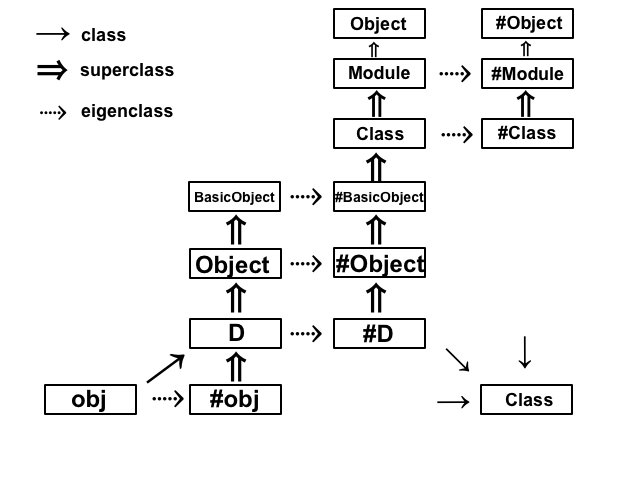
\includegraphics[width=1\textwidth]{figures/object_model.png}
\caption{Kompletní objektový model jazyka Ruby}
\label{fig:object_model}
\end{figure}
Eigenclass lze přeložit jako ,,vlastní třída objektu'' a odpovídá to tomu, kde tato třída skutečně je. Každý objekt (tedy i třída) má jen pro sebe kopii své třídy, ve které jsou definovány singleton metody. Teprve s touto znalostí můžeme zobrazit kompletní objektový model. Na obrázku \ref{fig:object_model} je zobrazena situace, kdy jsme si definovali třídu \emph{D} a vytvořili jednu její instanci, objekt \emph{obj}. Značení na obrázku by mělo být jasné. Když zavoláme metodu na objektu \emph{obj}, Ruby začne s vyhledáváním v eigenclass daného objektu a pokračuje vzhůru po předcích až k \emph{BasicObject}. Pokud zavoláme třídní metodu třídy \emph{D}, začne se vyhledávat u \emph{\#D} a pokračuje se opět až k \emph{BasicObject}.


\begin{thebibliography}{20}

\bibitem{rubysite}
  \emph{Oficiální web jazyka Ruby},
  \href{www.ruby-lang.org}{www.ruby-lang.org}

\bibitem{rubydoc}
  \emph{Oficiální dokumentace},
  \href{www.ruby-doc.org}{www.ruby-doc.org}

\bibitem{olsen2011eloquent}
  Russ Olsen,
  \emph{Eloquent Ruby}.
  Addison Wesley Proffesional Ruby Series, Massachusetts,
  2011.

\bibitem{metaRuby}
  Paolo Perrotta,
  \emph{Metaprogramming Ruby: Program Like the Ruby Pros}.
  Pragmatic Bookshelf,
  2010.

%\bibitem{metaTutorial}
%  Satish Talim,
%  \emph{Metaprogramming in Ruby},
%  \href{http://ruby-metaprogramming.rubylearning.com/}{online tutorial},
%  2011.

%\bibitem{continuations}
%  Loran Segal,
%  \emph{Demystifying Continuations in Ruby}.
%  \href{http://gnuu.org/2009/03/21/demystifying-continuations-in-ruby/}{personal blog},
%  2009.

\end{thebibliography}


\end{document}

